\scanpage{36}
\deleted{\[
f_X^*\bigl(\unsure{f_X^*}(X')\xrightarrow{\unsure{\operatorname{Fr}_{F/X}^*}}f_X^*(X')\bigr)
\]}
\deleted{$F_{X*}(F$}
\diagram{\begin{tikzcd}[column sep=large,row sep=large]
X' \arrow[d,"p"'] & X'^{p/X} \arrow[l] \arrow[d] & X'\,! \arrow[l,"\sim"',"\exists\text{ isom}" above] \arrow[ll,bend right=35,"f_{X'}" above] \arrow[dl,"p"]\\
X & X \arrow[l,"f_X"'] &
\end{tikzcd}}
\margin{\deleted{\unsure{?}}}
Peut-être que a) implique aussi b), en tous cas c'est vrai si on renforce a) en exigeant que $f_X$ garde la propriété \unsure{dite} après \uline{$\forall$} changement de base (en particulier le chgt de base $f_X:X\mathbin{-}X$ !).

Le prolongt de $\operatorname{Fr}_{X'/X}^*$ \inserted{$(X'\in\operatorname{Ob}X_{\text{ét}})$} aux faisceaux en $\operatorname{Fr}_{F/X}$ se \uline{caractérise}, \inserted{pour $X$ fixé}, par la \unsure{propriété} d'être fonctoriel en $F$ (et d'être un prolongt). Il est évidemment l'identité sur les faisceaux constants :
\diagram{\begin{tikzcd}[column sep=huge]
f_X^*(I_X)=I_X \arrow[r,"\operatorname{Fr}_{F/X}^*","\substack{\Vert\\\mathrm{id}_{I_X}}"'] & I_X
\end{tikzcd}}
comme on voit en se ramenant au cas où $I$ est réduit à un élément. On a \deleted{fonctorialité} compatibilité des $\operatorname{Fr}_{F/X}$ par chgmt de base \uline{quelconques}. La compatibilité aux chgmt de base étales, $+$ fonctorialité en $F$, suffit à le caractériser également -- \deleted{(\unsure{donc indépendance} de la \unsure{topologie} \unsure{de} $f_X$ !!!)}
\margin{\figure{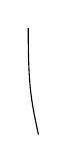
\begin{tikzpicture}\draw (0,0)..controls(0,-.7)and(.03,-.9)..(.13,-1.35);\end{tikzpicture}}}

Il induit l'identité sur les $H^0$, donc sur les $H^i$, $\mathrm R\Gamma_X$ $\cdots$
\mspage{35}
